\section{Evaluation}
\label{eval}

In this section we describe the evaluation of both the distributed and centralized experiments. Section~\ref{sec:data} explains the dataset in detail while in section~\ref{eval:dist} we explain the experiments setup of the distributed implementation along with the performance issues we faced. Section~\ref{sec:res} analyzes the experimental results.

\subsection{Data}
\label{sec:data}
We ran the affinity propagation algorithm in both a centralized and distributed manner. The data used to determine the sending pattern of different IP addresses is the same set of data used by SpamTracker~\cite{bb}. This data contains the received time of a given email, anonymized sender of the email, and the targeted domain, and lasts for a period of one month, from March 1st 2007 to March 31st 2007. In this dataset, some domains have not received many emails in the entire month of March. We removed domains that had received fewer than fifty emails in the entire month, leaving us with just over two hundred domains. 

To determine whether an IP address, that is currently not blacklisted (an \emph{accepted} IP address), is eventually blacklisted, we scan the rest of the dataset to check whether that IP address becomes blacklisted (a \emph{rejected} IP address) by the end of the month of March. Since we do not have ground truth nor a more accurate list to determine if the IP address becomes blacklisted in later months, this method can only detect a subset of true spammers.

\subsection{Distributed implementation}
\label{eval:dist}
Our distributed implementation was evaluated by running P2 on multiple Emulab~\cite{emulab} nodes. Emulab testbed can be used to emulate latency and bandwidth constraints to emulate real-world scenarios. We configured Emulab experiments to have a latency of 100 Mbps between nodes that emulate super-nodes. Currently, the distribution of IP addresses across super-nodes and the similarity calculations are done remotely. The super-nodes are given the similarity information as input.

Due to a bug in P2 we were not able to perform experiments on more than 5 nodes that have a total of 30 IP addresses to cluster. The bug in P2 caused outgoing network messages to get queued up and sent after long delays. Affinity propagation was sending approximately 60 messages from a node to multiple remote nodes during each iteration. We had to keep the epochs of 10 seconds in order to get all messages picked-up from the internal queue of P2 and sent to the destination.

We were able to cluster approximately 3500 spammers out of the initial 6 hours using random sampling and greedy clustering. The score distribution of the next six hours accepted/rejected IP addresses classified using this result is discussed in section~\ref{sec:res}. We also evaluated the distributed implementation by comparing the clusters from the distributed experiments with the results of centralized implementation of the affinity propagation (implemented in MATLAB). We found that the distributed implementation gave exactly the same clusters. 

For the centralized experiments, the IP addresses were split within the \emph{$\bigtriangleup t$} time interval due to MATLAB's memory constraints. However, the greedy approach was not used, as the need to reduce the number of runs of centralized affinity propagation is not needed. The matlab implementation\footnote{This implementation is free to view and download at \url{http://www.psi.toronto.edu/affinitypropagation/}} of affinity propagation that we used was developed by Frey and Dueck~\cite{affinity}.

\subsection{Results}
\label{sec:res}

Figure~\ref{fig:distScores} shows the distribution of scores for both the list of \emph{accepted} and \emph{rejected} IP addresses in the distributed experiments. The same graph is shown in figure~\ref{fig:centScores} for the centralized run of affinity propagation using the complete set of IP addresses for a six hour period. The classification phase from the distrusted experiment clusters give score of smaller magnitude. This is due to the cluster information not being as rich as in the centralized experimental run (due to using a smaller number of IP addresses in the experiments), the patterns in the score distribution are similar to each other and to the results in \cite{bb}. \emph{Rejected} IP addresses tend to have larger scores as these IP addresses are known spammers, and have similar sending patterns to other spammers. \emph{Accepted} IP addresses have smaller scores, and we suspect that \emph{accepted} IP addresses with scores greater than five, are spammers that have yet to be blacklisted. 
\begin{figure}[t]%{4.25in}
\centering
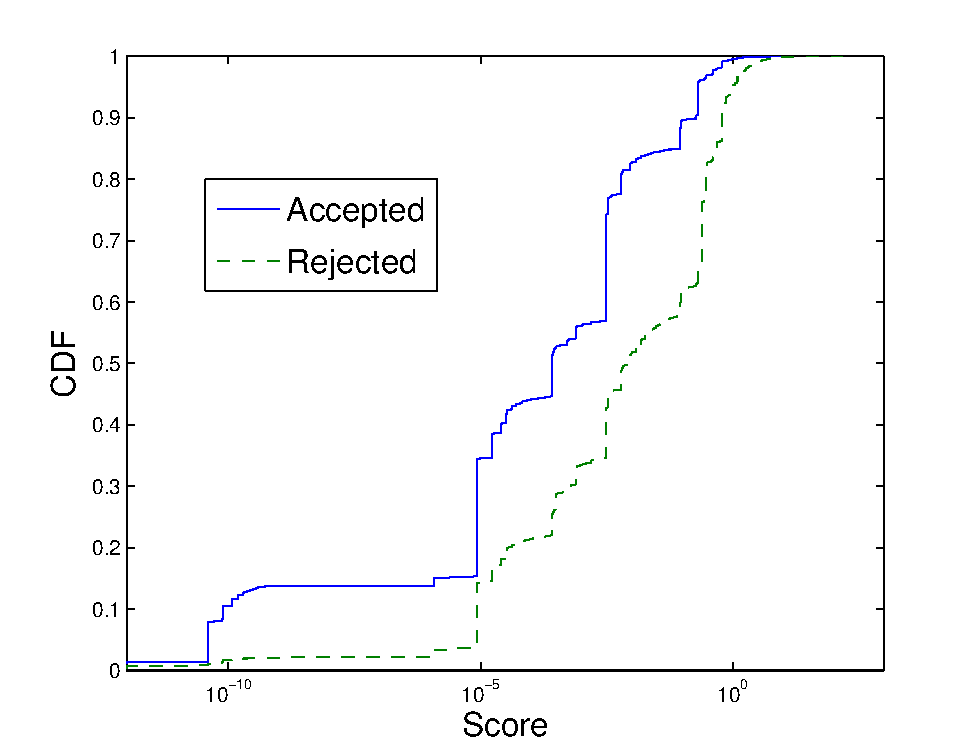
\includegraphics[width=0.45\textwidth]{figures/distScores2}
\caption{The distribution of scores for the small distributed experiment, after classifying IP addresses that send email in the next six hours to any of the domains. The blue solid line represents the \emph{accepted} IP addresses and the green dashed line represents the \emph{rejected} IP addresses. }
\label{fig:distScores}
%\vspace*{-5mm}
\end{figure}

\begin{figure}[t]%{4.25in}
\centering
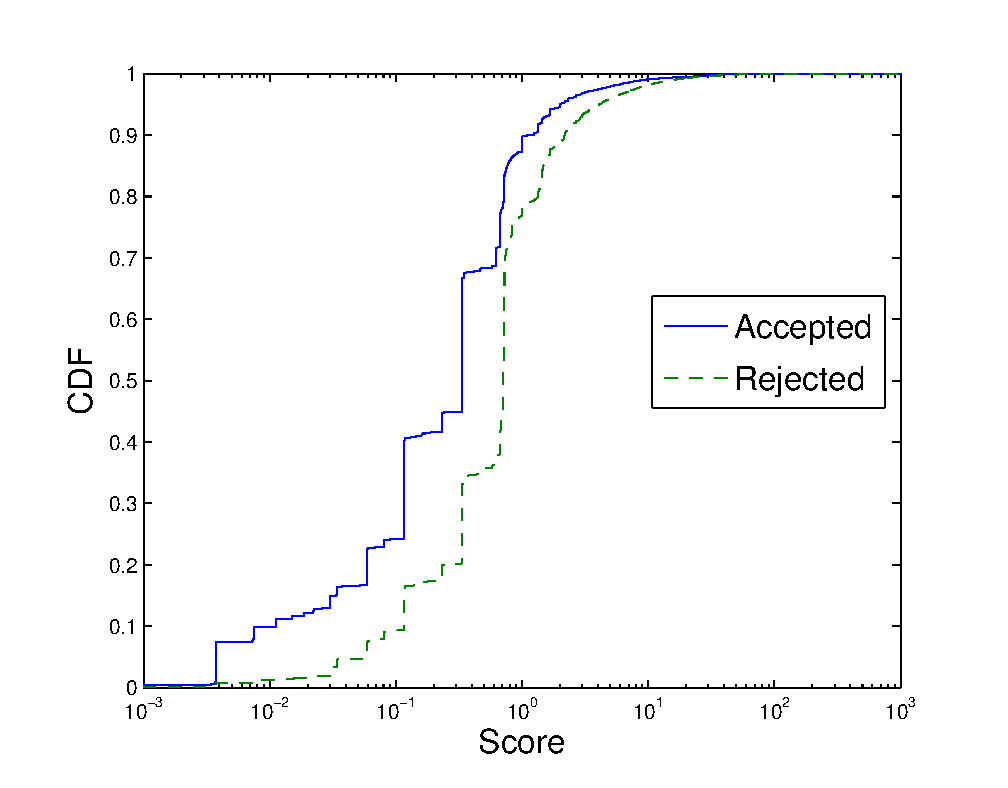
\includegraphics[width=0.45\textwidth]{figures/centralScores2}
\caption{The distribution of scores for the centralized experiment, which uses the entire data in the six hour time interval, after classifying IP addresses that send email in the next six hours to any of the domains. The blue solid line represents the \emph{accepted} IP addresses and the green dashed line represents the \emph{rejected} IP addresses.}
\label{fig:centScores}
%\vspace*{-5mm}
\end{figure}

To better test our hypothesis, we ran more complete experiments in a centralized manner to avoid the performance issues in P2. In these experiments, we first ran a single round of clustering for a six hour time interval. We combined the cluster averages, which were generated from the six hour interval, with the next six hours to generate a new set of clusters using affinity propagation. This is repeated until we covered a time period of 15 days, from March 1st 2007 through March 15th 2007. 

Our results indicate that almost 30\% of the \emph{accepted} IP addresses that become rejected later on, have scores that are greater than five. In SpamTracker~\cite{bb}, only 10\% of the \emph{accepted} IP addresses that are actually spammers are found. However, our results are not strictly better than the results found with SpamTracker~\cite{bb} despite the fact that it appears we capture more of the true spammers. Since we only have a subset of IP addresses that are initially \emph{accepted} that are later \emph{rejected}, we are likely overshooting the true percentage of these spammers that our implementation detects. However, we only cluster the first fifteen days, and there may be additional spamming sending patterns that are only revealed in the latter fifteen days of March. 

Of the scores that are greater than five, less than ten percent of these are IP addresses that never get rejected later on during the month of march. Thus, the maximal bound of false positives is ten percent, and we suspect that many of these IP addresses are in fact spammers that were not blacklisted by the end of the month. Much like SpamTracker, this method of determining which IP addresses are spammers should be used in addition to existing methods to find additional spam email that current filters miss. 
